% Created 2024-04-20 Sat 06:09
% Intended LaTeX compiler: pdflatex
\documentclass[11pt]{article}
\usepackage[utf8]{inputenc}
\usepackage[T1]{fontenc}
\usepackage{graphicx}
\usepackage{longtable}
\usepackage{wrapfig}
\usepackage{rotating}
\usepackage[normalem]{ulem}
\usepackage{amsmath}
\usepackage{amssymb}
\usepackage{capt-of}
\usepackage{hyperref}
\usepackage[margin=1.0in]{geometry}
\usepackage{draftwatermark}
\author{Perry Kundert}
\date{2024-04-16}
\title{Business Plan for Local Currency Deployment}
\hypersetup{
 pdfauthor={Perry Kundert},
 pdftitle={Business Plan for Local Currency Deployment},
 pdfkeywords={},
 pdfsubject={},
 pdfcreator={Emacs 29.1 (Org mode 9.6.10)}, 
 pdflang={English}}
\begin{document}

\maketitle
\begin{ABSTRACT}
Money created through debt and centrally-managed through interest rates has proven to be
problematic.  The benefits the ability to create and issue large amounts of money to fund projects
are overwhelmed by the caustic effects of inflation, and the exponential growth of interest
obligations.

Issuing fungible and trustworthy asset-backed money based on individual or collective wealth has
until now been out of reach.  The technical hurdles, and the opposition of entrenched political and
banking incumbents have been insurmountable.

The time has now arrived where we are able to surmount these obstacles:
\begin{itemize}
\item Technology to implement reliable and performant decentralized monetary systems is here.
\item The public will to accept decentralized value-stable money is rising.
\item The government and bank opposition to sound money can be legally and technically overcome.
\end{itemize}
\end{ABSTRACT}

\setcounter{tocdepth}{3}
\tableofcontents

\section{Executive Summary}
\label{sec:org141ae1a}

The widespread use of alternative sound money hinges on solving three problems:

\begin{enumerate}
\item Paying and accepting sound money in realistic, non-ideal circumstances.
\item Creating units of sound money dynamically, without central authority.
\item Improving the definition and implementation of sound money over time.
\end{enumerate}

\section{What is "Sound Money"}
\label{sec:orgcdd9990}

\begin{quote}
"The gold standard makes the determination of money's purchasing power independent of the changing
ambitions and doctrines of political parties and pressure groups. This is not a defect of the gold
standard; it is its main excellence." -- Ludwig von Mises
\end{quote}

Reliable convertability of money to something of value -- resistance to debasement -- is a major
(often subconscious) requirement users have of Sound Money.

Some methods result in wealth being exchanged for units of money:

\begin{enumerate}
\item Directly using the valuable commodity as money (eg. gold coinage, barter)
\item Trusting some central authority to issue/redeem money for some valuable commodity (eg. gold-backed money)
\item Exchanging wealth for some other money with certain desirable properties (eg. Bitcoin, Fiat currency)
\end{enumerate}

These are all analogous to "selling" wealth for money in Fiat banking.  The wealth owner loses
access to the wealth, gaining only the money (or what it purchased).  This is typically the only
form of money ownership available to the general population.

Alternatively, the creation and attested ownership of wealth can produce money; the owner retains
use of the wealth, and units of money are created (which must be redeemed, in order to sell or
transfer the attested wealth):

\begin{enumerate}
\item Using money representing confirmed ownership of wealth (eg. securitization, tokenization)
\item Creation of credit balances of money in Mutual-Credit systems.
\end{enumerate}

These are mechanically very similar to "borrowing" in Fiat banking terms; a lien is established on
the underlying wealth, various guarantees are assured (insurance, proof of title, etc.), and the
credit balance is created.  The balance created must be returned if the wealth is sold, or
destroyed (triggering insurance).  This type of money ownership is primarily reserved for the
elites, except at very onerous terms and high interest rates (eg. Mortgages, demand loans).

Most oddly; the issuers of these loans (commercial banks) create these deposits out of thin air;
they have no collateral other than that provided by the borrower.  In return for this amazing
government-mandated monopoly, they can charge interest for creating these new units of money.

\subsection{Sound Money vs. Debt Money}
\label{sec:org63801a0}

All of these forms of Sound Money have a couple of significant deficiencies vs. debt-created Fiat money:

They are typically not \emph{fungible}; "tokenized" chickens have a different value than some "mutual
credit" units or "silver" coins.

As a consequence, accumulation of large pools of money is very challenging.  Any large pool
consists of various types of money, with a dynamic value vs. each other, and also vs. the
acquisition target of the pool.

Debt-created Fiat money, on the other hand:
\begin{enumerate}
\item Is fungible; all assets are converted into money, which can be pooled interchangeably.
\item Is easily created; bonds can be issued and sold in large markets to raise funds.
\end{enumerate}

While a Fiat money supply retains its convertability to wealth, this works well.  But typically,
such convertability ceases as soon as the politicians controlling the treasury and central bank
can manage it.

As a final result, the Cantillon Effect produces a fountain of unbacked money the flows through
the hands of those closest to the treasury and central bank, allowing them to purchase wealth
with current dollars, while the ultimate sellers end up with debased dollars in exchange.

\subsection{Competitive Sound Money}
\label{sec:orgb98c24b}

All of these forms of money creation will continue to be available.

We propose making the creation of Sound Money available to the general public, through the
attested ownership of wealth, without interest -- completely out of the control of central
planners.

The public can choose to take their collateral wealth and sell, convert or lend it to create
traditional forms of money, if they so choose.

But, by making it possible for the general public to create balances of value-stable wealth-backed
money on demand without interest (through the attested ownership of wealth and assurance of
guarantees), it is likely that they will quickly convert any available wealth to sound money, and
pay down their interest-bearing debt.

\section{Proposed Transition}
\label{sec:org12c0cdb}

\subsection{Establish Non-Fiat Payment Options}
\label{sec:orgc953d65}

Immediately prepare and begin to roll out:

\begin{enumerate}
\item Cryptocurrency based payment rails for both vendors and and buyers.
\item Recommend ongoing pricing in Gold \& silver coin.
\end{enumerate}

All non-Fiat savings can be hedged against conversion loses in the traditional Fiat futures or
options markets, if necessary to protect future Fiat denominated obligations.

\subsubsection{Crypto Wallet Setup, Security \& Reliability}
\label{sec:org9b885de}

\subsubsection{Crypto L2 Payments}
\label{sec:org822b085}

\begin{enumerate}
\item Bitcoin "Lightning"
\label{sec:orgad68bc5}

\item Ethereum Roll-Ups
\label{sec:org72ae15c}
\end{enumerate}

\subsubsection{Precious Metals}
\label{sec:orge732543}

\subsubsection{Barter}
\label{sec:orgff70e87}

\subsection{Develop Mutual Credit Community Based Money}
\label{sec:org2005095}

We propose developing a Holochain-based framework for deploying community-based Money.  Credit balances will  be created
directly through the community's attestation of wealth (proof of traditional valuation, insurance and liens).

\subsubsection{Insurance}
\label{sec:org15716bb}

The insurance required to assure the integrity of the community money may be provided by external
insurers, or may be provided by the money's authoring community for a fee.  It should reflect the
actuarial risk of the assets (a car on the road vs. silver in a bank safe deposit box), the net
balance of the account (proportion of the asset value being insured), and the risk of the owner
(historically how likely is such an owner to default, defraud, etc.).

These estimation techniques are widely known in the risk community, and should be adjusted from
time to time to ensure stability of the insurance fund.

The triggering of payouts from the fund should be prompt, to maintain the net zero balance of the
mutual credit currency.  They may be automatic (eg. triggered after a certain threshold and/or
time period of negative balance), or manually triggered, as desired by the community money's
organizers.  However, valid mutual-credit operations in process must remain valid, so long as
they were entered into before the account fell into arrears.

\subsubsection{Convertability}
\label{sec:orgbe17227}

Conversion to other Cryptocurrencies and to/from Fiat is accomplished through integration into the
existing Ethereum ERC-20 DeFi exchanges platforms (eg. Uniswap).

A centralized community exchange controls conversion between Mutual Credit units and ERC-20 units
on a one-to-one basis.  This would be run by the same community organization in charge of the
attestation of wealth underpinning the community mutual-credit currency.

\subsubsection{Value Stability}
\label{sec:orga69a78b}

If desired, the definition of the community currency can be defined to be value-stable in terms
of some reference basket of wealth.

When wealth is pledged to create a credit balance, the process is:

\begin{enumerate}
\item Estimate the value of the wealth in its primary market (eg. USD\$)
\item Estimate its assets' uncertainty function over time (eg. reduced value since attestation).
\item The community responsible attests to the wealth, and the presence of necessary insurances.
\item Apply the money's current credit multiplier to compute the credit balance, reduced by the
uncertainty function, regularly (eg. daily or hourly) on all credit balances.
\end{enumerate}

A closed-loop control function (such as a PID loop) measures and corrects money unit/basket value:

\begin{enumerate}
\item The current value of the proposed wealth basket (eg. in USD\$/basket, in their markets)
\item The current value of the community money (eg. in USDC/unit, on DeFi exchanges)
\item The control function computes the new money credit multiplier due to in/deflation
\item All credit balances are adjusted due to the new credit multiplier
\item Any accounts with negative credit balances must attest more wealth, or purchase money on the market to restore net positive balance.
\item Insurance contracts are executed to make good any account persistently in arrears, using traditional means to recoup losses.
\end{enumerate}

\section{Financial Projections}
\label{sec:orgf2130c0}

We propose an aggressive R\&D plan over a 1 year period, resulting in several prototypes followed
by an operational deployment of a Holochain-based community money system.

\subsection{1st Year: \$1,000,000 Cost}
\label{sec:orgeef3426}

Over the first year, R\&D and community communications and collaboration are costs, with no income
from system operations to offset them.

\subsubsection{Initial R\&D: 6 Months}
\label{sec:org3c474db}

I foresee the first 6 months of the year dedicated to:

\begin{enumerate}
\item Designing and testing currently available near-term systems and solutions such as Lightning Network
\item Producing PR and travelling extensively to communicate the long-term plan, and advise on near-term solutions.
\item Producing 2-4 prototypes of the community money system, with increasing functionality
\item Designing an integration with traditional insurers to provide re-insurance
\end{enumerate}

\subsubsection{Operational Deployment: 6 Months}
\label{sec:org3a65231}

Once an operational mutual-credit community money system is accepted, and the community money
ERC-20 exchange is operational, initial deployment can begin.

A small set of vendors with some large willing clients is chosen, to invest a subset of their
trade through the community money system.  Instead of settling in cash, the clients either
create community money (through attestation of wealth) or purchase it using the Fiat USDC to
ERC-20 token DeFi, then exchange for mutual credit units via the community exchange.

Then, they settle client to vendor transactions using community money instead of Fiat.

Finally, the vendor cashes out community money via the community money to ERC-20 exchange, and
then the ERC-20 DeFi pool to receive USDC, when can be converted and deposited to Fiat accounts
via any Cryptocurrency exchange.

Alternatively, the vendor can purchase wealth using community money payments to other vendor(s).
Then, by attesting the newly purchased wealth, they can create new community money (interest
free), and cash that out, as described above.

\subsubsection{Technical Team Lead: \$200,000}
\label{sec:orgbf1bccf}

\subsubsection{Holochain Full-Stack R\&D: \$200,000}
\label{sec:org65a99e5}

\subsubsection{Monetary System R\&D: \$200,000}
\label{sec:orga9d4d96}

\subsubsection{Community Interface \& Product Owner: \$150,000}
\label{sec:orga19427a}

\subsubsection{Social Media, Communications \& PR: \$100,000}
\label{sec:orgf7a7a5e}

\subsubsection{Hardware, Software: \$50,000}
\label{sec:orgbf6e03a}

\subsubsection{Travel, Misc. Expenses: \$100,000}
\label{sec:orgdec92c4}

\subsection{2nd Year: Neutral}
\label{sec:orgc3419a3}

Wider community uptake results in insurance fee revenue collection filling the loss buffer, and
sufficient to pay for maintenance and further R\&D of the operating community money system.

\subsection{3rd Year: Profitable}
\label{sec:orgf76317c}

Fees on wealth attestation insurance begin to stabilize, and are automated using PID control to
yield a revenue stream to support the ongoing operations of the community money system, while
maintaining a buffer against adverse insurable events (eg. natural disasters)

{\scriptsize
\begin{center}
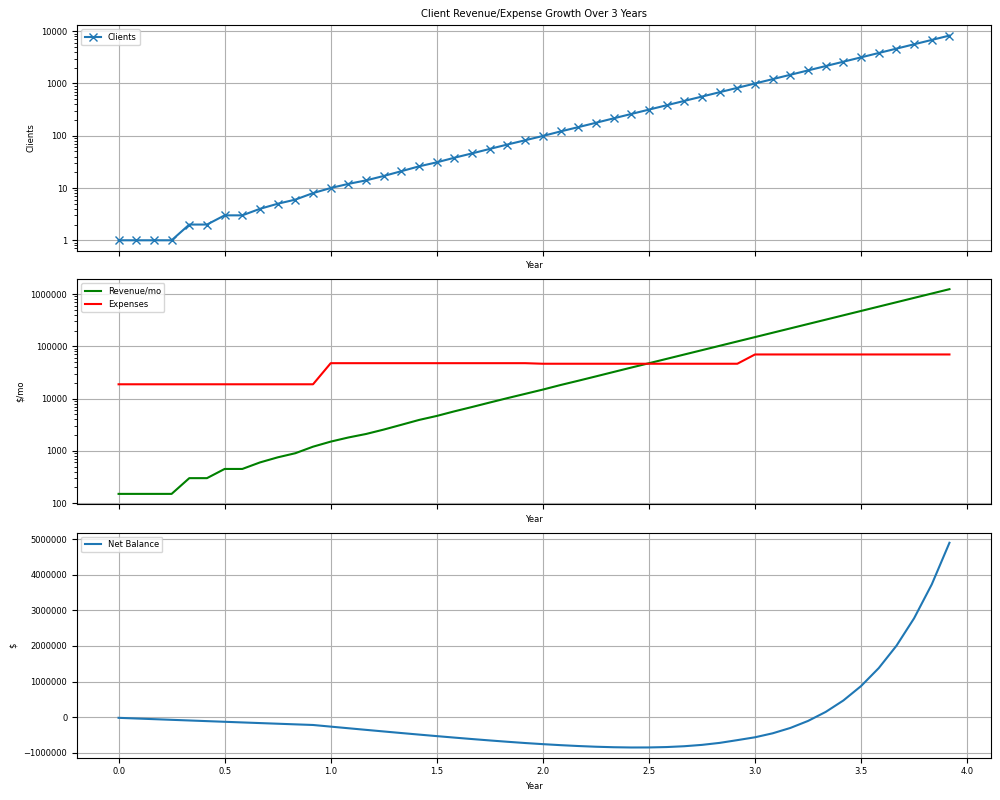
\includegraphics[width=.9\linewidth]{images/revenue-projection.png}
\end{center}

}

\section{Conclusion}
\label{sec:org396e050}

An aggressive plan to develop a viable mutual-credit community currency is proposed.

A 1-year plan to research, develop, deploy and test the community money system establishes a group
of vendors and clients to test the prototype deployment using real money, in preparation for the
second year's opening of the system to further vendors and clients, who can either purchase or
create community money through attestation of wealth.

Let's build this future together.
\end{document}